\chapter{Trials}

\section{Definition Of Freetrials Competitions}
The object of Freetrials is to ride over obstacles. 
A Freetrials competition takes place on a ``course'' containing different obstacles called ``sections''. 
Each section is worth one point, and courses typically contain 15 – 40 or more sections.

Riders earn points by successfully riding (``cleaning'') each section from start to finish. 
The objective is to earn as many points as possible by cleaning as many sections as possible.

At the end of a specified time period, the rider with the highest overall number of points (who has cleaned the most number of sections) is the winner.

\section{The Course}
The competition takes place within a specified time period (2+ hours depending on the number of obstacles), on a collection of 15 to >40 independent, numbered sections of any length (typically 3 m to 20 m long). 
Sections may include narrow beams or logs, steep climbs, rocks, etc.

The average difficulty level of sections will vary between competitions depending on the ability level of the riders participating. 
In all competitions, section difficulty should be evenly represented at all levels from the most beginner to the most expert riders. 
See Appendix 1 for more information on setting sections. %ref

At each section are posted instructions that identify the section number, its difficulty level, and a description of the section.
Section boundaries are defined by flagging tape and/or instructions that designate a start line, section boundaries, and a finish line.

\section{Competition Time Duration}
The competition time duration is based on the number of obstacles and competitors. 
The typical time duration is 2 hours with an approximate formula of 2-3 minutes per obstacle to allow each rider time to attempt each obstacle multiple times, if necessary. 
The size of the course, number of sections, and number of riders competing at one time can also factor into the time duration of the competition.

All riders must stop riding at the end of the time limit. 
If a rider is mid-way through an attempt when the time limit is reached, they are allowed to finish that attempt.

\section{Competition Categories}
Competitors are divided up into different categories for the purpose of awarding prizes. 
Rider age groups should include 0-14, 15-29 and 30-UP as the minimum. 
Depending on the host, additional breakdown of ages could be used (for example:0-12, 13-14, 15-19, 20-29, 30-39, 40-UP). 
The age groups should also be split male and female with a minimum of 6 (3) riders in a group following 1.2.2. %ref
Due to the size of the course and the number of competitors, the competition may be split into several time slots. 
Splitting the time slots by age group is preferred. 
Competitors who think they have a chance at the final competition should be in the same time slot and indicate this preference on the registration form.

\subsection{Final Round}
When the competition has been completed, the top riders for male and female would compete in the final round for the championship.
The minimum number of top riders would be 6 for each male and female with the upper limit up to the host. 
There should be at least 6-10 additional lines that represent the difficulty of the top riders. 
Male and female finalists may have different lines depending on the overall ability of each gender.

In the finals, long lines with multiple skills can be built completely new or combined from existing lines which were used in the preliminaries. 
The host should take attention that the lines for the final are close together and on a place that is good for spectators. Depending on the used obstacles, there should be 20 - 30 minutes of competition time for each group. 
Between the competition and the final should be a minimum of a 1-hour delay, or on another day.
 
\section{Section Restrictions For Competition Categories \label{sec:trials_section-restrictions-for-competition-categories}}
Normally, all riders of all categories are free to attempt any sections they wish, in the entire course.

In cases where there is a wide range of rider ability, or if there are space or time restrictions, the Event Director may use the following system which allows the top level riders to skip the sections that were set for beginner riders.

The sections must be sorted into ``blue'' (beginner lines), ``red'' (midrange lines), and ``black'' (Pro lines). 
Each line should be marked with one of these colors. 
A dot (on the section description card) is acceptable, but it is recommended to color the complete line marking in the fitting color. 
Also on the judging paper the rider had to find all line numbers with the right color then to get an easy overview what to do.

All riders that successfully ride all the red lines will automatically receive the points from all the blue lines.
Blue, red and black should be divided in the following way.
\begin{itemize}
\item Blue lines are all obstacles that require jumps up to two pallets high (30cm), with a low technical skill, and/or gaps less than 40cm.
\item Red lines are with jumps from three to six pallets high, and/or technical difficult sections (for example: small rails, difficult angles...). The gaps can be up to 1.20m.
\item Black lines require jumps from seven pallets or higher, technical very difficult installations, gaps from more than 1.20m, deep drops, and so on. 
\end{itemize}
A typical course should provide up to 25 blue lines, 50 red lines and 25 black lines.


\section{Scoring Points}
Each section is worth one point, and the objective is to score points by successfully riding (``cleaning'') as many sections as possible within the specified time period.

\subsection{Definition Of ``Cleaning''}
Cleaning a section is defined as follows:

\begin{enumerate}
\item \textbf{Riding into a section.} This is defined as the moment a rider's front axle crosses over the start line.
\item \textbf{Riding through the section without ``dabbing''.} Dabbing is defined as follows:
	\begin{enumerate}[a.]
	\item Allowing any part of the rider's body to touch the ground or obstacle. 
	If loose clothing brushes against the ground or obstacle but does not influence the rider's balance, then this is acceptable (does not constitute a dab).
	\item Allowing any part of the cycle except the tire, rim, spokes, crank arms, pedals, bottom bracket, bashguard or bearing housings to touch the ground.
	\item Riding or hopping outside the boundaries of the defined section.
	The axle(s) of the cycle must be within the boundaries of the section at all times, even if the rider is in the air (e.g., a rider cannot hop over a section boundary that turns a corner, even if they land back inside the section).
	\item Breaking the flagging tape or other markers that are delineating a section boundary. 
	Touching or stretching the tape does not constitute a dab, as long as the axle(s) remain inside the section boundary.
	\item Riding a section in any way that is not consistent with the instructions outlined for that problem.
	\end{enumerate}
\item \textbf{Exiting the section.} A rider exits a section when their axle(s) fully cross over the finish line, or are within a
defined finish area (such as a taped circle on top of a boulder). 
There is no requirement to exit in control.
If a rider falls across the defined finish line but manages to exit without dabbing, they have cleaned the section.
\end{enumerate}

\subsection{Exceptions And Special Notes}
When hooking a pedal on an obstacle, it is acceptable for a rider's heel and/or toe to initially contact the ground, as long
as most of the rider's foot is still on the pedal. 
However, after a rider is established in position, weighting the heel or toe on the ground constitutes a dab.

It is acceptable for a rider's body to be entirely on one side of the centerline of the cycle.
Riders may attempt any problem multiple times until they succeed or decide to abandon the section.
However, it is not possible to earn additional points by cleaning a section more than once, and no points are awarded if the rider does not clean the entire section.

If there is a lineup for a section, the rider must go to the end of the line after each attempt.

\section{Observers}
Observers are responsible for judging whether a rider has successfully cleaned a section. 
There are several possible ways for an Event Director to organize Observers at an event:
\begin{itemize}
\item One Observer can be assigned to judge at each section. 
This is the best option but is normally not possible because there are normally more sections than Observers.
\item Each Observer can be assigned to judge several sections in the nearby vicinity. 
In this case, it is the responsibility of the rider to ensure that an Observer is watching when they attempt a section.
\item Riders can be split into groups, and one Observer is assigned to each group. 
This Observer would then follow the group around as they go from section to section.
\item At small events, there may not be a need for Observers. 
Riders waiting to attempt a section may serve as Observers for the rider who is currently attempting the section. 
This is termed ``self-judging'', and it is up to the riders to ensure that scores are honestly recorded. 
This is the most common method for smaller competitions.
\end{itemize}

\section{Keeping Score}

\subsection{Method 1}
Method 1 is mandatory for all major competitions and is the recommended method for all other competitions.

Each rider is issued a scorecard (see example) at the beginning of the competition, and must give their card to an Observer prior to attempting a section.
If the competition is self-judged, the rider attempting the section gives their card to another rider who must observe them attempt the section.
If they clean the section, the observer indicates that they have completed the section by initialing or punching the box corresponding to that section. 
At the end of the competition, riders hand in their cards to the Event Director or to a designated person for tallying of scores.

\textbf{Example scorecard:}

\begin{tabular}{|l|l|l|}
\hline 
\textbf{Rider Name:} & \textbf{Category:} &  \\ 
\hline 
Section Number  & Section Number  & Section Number \\ 
\hline 
1 & 6 & 11 \\ 
\hline 
2 & 7 & 12 \\ 
\hline 
3 & 8 & 13 \\ 
\hline 
4 & 9 & 14 \\ 
\hline 
5 & 10 & 15 \\ 
\hline 
\end{tabular}

\subsection{Method 2} 
This method is intended for small events, and is not appropriate for larger events. 
Major events such as Unicon or national meets must not use this system of scoring.

In this method, one or two observers keep track of scores for numbered sections on a computer or paper spreadsheet such as this:

\begin{tabular}{|c|c|c|c|c|c|c|c|c|c|c|c|c|c|c|c|}
\hline 
 & \textbf{Section:} & & &  & &  &  &  &  &  & & & &  &   \\ 
\hline 
\textbf{Rider} & \textbf{Category} & 1 & 2 & 3 & 4 & 5 & 6 & 7 & 8 & 9 & 10 & 11 & 12 & 13 & 14 \\ 
\hline 
Jane Smith & Expert &  &  &  &  &  &  &  &  &  &  &  &  &  & \\ 
\hline 
John Anderson & Sport &  &  &  &  &  &  &  & &  &  &  &  &  &  \\ 
\hline 
 &  &  &  &  &  &  &  &  &  &  &  &  &  &  & \\ 
\hline 
 &  &  &  &  &  &  &  &  &  &  &  &  &  &  & \\ 
\hline 
\end{tabular} 

After cleaning a section, riders must return to the Observer and tell them which section they cleaned.

\section{Participation By The Course Setter(s)}
Due to the grassroots nature of many events, the course setter(s) are allowed to compete. 
Although the course setter may initially be more familiar with course sections than the other riders, this should not result in an advantage because everyone is allowed multiple attempts to complete sections. 
However, if the Course Setter(s) chooses to also compete, they must conform to Rider Responsibility ``F'' (see section ) and refrain from riding on the course prior to the competition, including while they are designing and building the sections. %ref

\section{Safety}
All riders must wear appropriate safety gear, such as helmets, shin and knee protection and gloves or wristguards.
Dangerous sections must not be constructed, and in particular, there should be no dangerous objects to land on if a rider falls off a high object. 
Artificial sections should be constructed so that they do not collapse or fall over under normal riding conditions.

If an Observer or the Event Director feels that safety is compromised by a rider attempting a section that is beyond his/her
ability, they may prohibit the rider from attempting that obstacle. 
In cases where a fall from an obstacle could be particularly dangerous, the Event Director may also permit attempts only by highly skilled riders who believe they will qualify for the Finals.

\section{Rider Responsibilities}
\begin{itemize}
\item The rider must know the rules.
\item The rider must gauge their time. 
No allowance will be made for riders who spend too much time at one obstacle and cannot complete the course before the end of the competition time period.
\item The rider is responsible for knowing where a section starts and ends, and which route he or she is supposed to take.
\item If two or more sections overlap, it is recommended that only one rider at a time attempt any of the overlapping sections. 
If two or more riders are on overlapping sections at one time, the rider who started first has the right-of-way.
\item The rider is responsible for his or her scorecard. 
If it becomes damaged, the rider can ask the Event Director for a new one. 
If it becomes lost, the rider will be issued a new card but their score will return to zero.
\item No rider may attempt any obstacle prior to the start of the competition. 
Ideally there should always be a separate practice area set up outside the competition area, for warming up prior to competing.
\item Intentional modification of a section by riders or spectators is prohibited. 
Note that kicking objects to test stability does not constitute intentional modification if an object moves. 
If a section is unintentionally modified or broken by a rider, they should inform the Event Director or Course Setter who will return the obstacle to its original form if possible.
\end{itemize}

\section{Protests And Dispute Settlement}
A protest can be lodged by anyone against an Observer's ruling. 
Protests typically arise when a bystander (another rider, or a spectator) observes a rider make an infraction that is not recorded by the Observer, or when an Observer gives the wrong penalty.

Protests must be lodged with the event director within fifteen minutes of the official results being posted. 
Protests must be in writing, and must note the rider, and section number and a description of the protest.

For small-scale events, the Event Director can act as the sole jury member. 
For larger events there should be a Jury consisting of at least three members, and they should be appointed in advance of the event. 
The Jury should be composed of the Event Director, the head Observer or Event Commissar if applicable, and a riders' representative. 
If there is no head Observer, the Event Director can appoint any person with experience in trials. 
Care should be taken to avoid conflict of interest and, in the event that a protest involves someone close to a Jury member, that person should be replaced for evaluation of the protest in question.

The jury will base its ruling on the input from the relevant parties, including the rider, the Observer, and the person who lodged the protest.
In the evaluation of protests, the benefit of the doubt must go to the Observer. 
The Jury is not obliged to overrule the Observer based on testimony from witnesses. 
Only if all parties present at the incident agree on the facts, and the Observer accepts that he or she made an error in assigning penalties, can an Observer's decision be overturned.

\section{Tie Breaking}
A tie occurs when the competition finishes and one or more riders have completed the same number of sections.
The Course Setter should collaborate with the tied riders to create a new, ``tiebreaker section'' at an appropriate level of difficulty. 
This section should be relatively long and may consist of several existing sections joined together, or an entirely new section.
The section should contain obstacles of increasing difficulty towards the exit location.

Each tied rider attempts this section and the winner is the person who rides the furthest without dabbing.
Only one attempt is allowed. 
The furthest location of a rider is defined by the part of the cycle that is touching the ground (the crank, pedal, or tire), prior to dabbing. 
There is no requirement for the rider to be in control. 
For example, if a rider lands a drop onto their tire, but immediately dabs, their furthest point would be the location where their tire last touched prior to dabbing.
If more than one rider cleans the tiebreaker section, another tiebreaker should be conducted with a more difficult section.

\section{Cycle Design Restrictions}
Any unicycle may be used. 
There is no restriction on changing unicycles during the competition.

\section{Guidelines For Course Setters}

\subsection{Numbering And Describing Sections}
Course setters should ensure that they have the following material for flagging and describing sections: flagging tape, duct tape, spray-paint, a staple gun, paper or cardboard, a felt marker, and large size Ziploc bags. 
Laminated cards with large letters A, B, C, etc. or 1, 2, 3, etc. are also very useful for labeling obstacles for description purposes.

Each section must be clearly numbered and have clearly marked start and finish locations. 
Be especially careful to clearly define the finish so it is clear when a rider has cleaned a section.

Assigning difficulty ratings to sections is not required. 
However, it is recommended that difficulty ratings be assigned to sections and listed on the rider scorecards, because it allows riders to quickly determine which obstacles they wish to attempt. 
If the restriction system described in section \ref{sec:trials_section-restrictions-for-competition-categories} is used, difficulty ratings on obstacle and scorecards are a must. 
For international competitions it is recommended to add section instructions to each line. 
Those should include the following information:

\begin{enumerate}
\item  Start: Description of the start location
\item Section: Description of the section and section boundaries
\item Finish: Description of the finish location
\item Sketch of the section (optional)
\end{enumerate}
Using sketches is strongly recommended cause all riders do not speak the same language. 
In some cases it can replace written instructions.

\textbf{Example Instructions and Sketch:}

\begin{tabular}{|p{8cm} r|}
\hline
\vspace{1mm}
\textbf{Section 22}

\textbf{Start:} Between the yellow tape, onto Beam A

\textbf{Section:} Ride from Beam A onto Spool 1, then to Box 2.

\textbf{Finish:} Ride off Box 2, staying between the 2 lines of flagging tape.
\vspace{8mm}
&
\raisebox{-1\height}{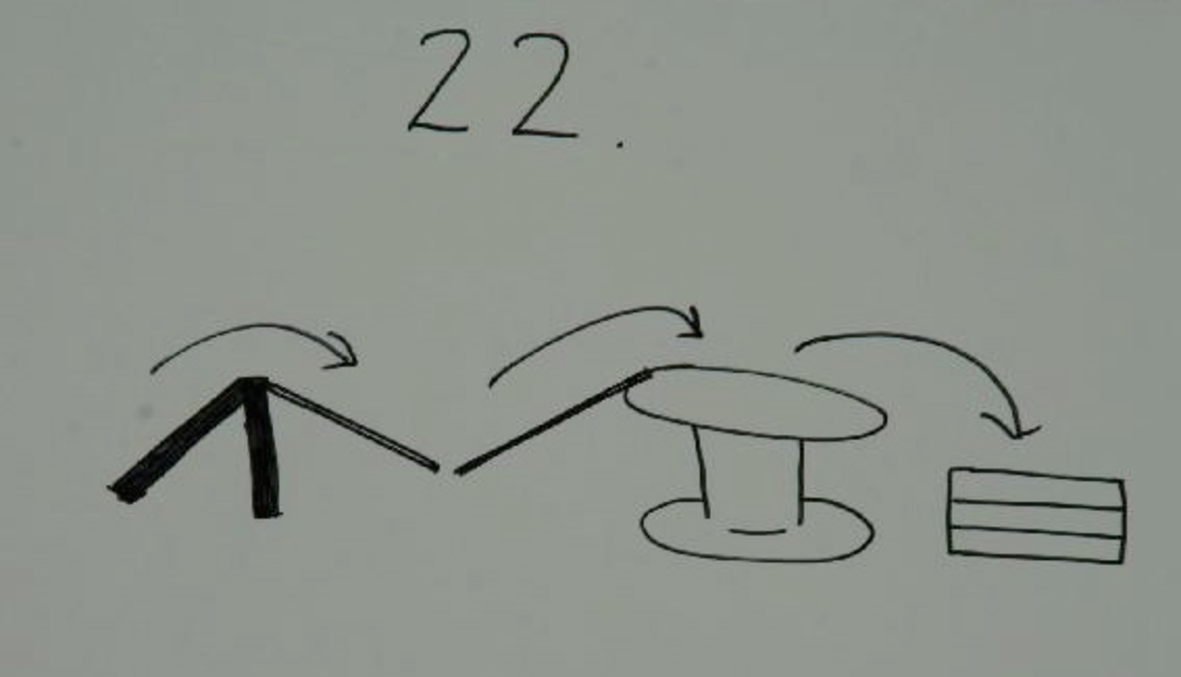
\includegraphics[scale=0.3]{trials} }\\
\hline
\end{tabular}

To make it easier to describe sections, label major obstacles with numbers and/or letters. 
These should be clearly visible at a distance. 
Plastic laminated cards with letters or numbers are good because they can be re-used at other competitions.

One good strategy is to label all boxes with numbers, and all beams with letters. 
This makes it much easier to include section descriptions such as ``ride from Beam A to Box 6, without touching the ground.''
Section instructions should not require or prohibit a rider from using certain techniques to complete a section. 
For example, the instructions must not prohibit the use of pedal grabs or bash guards in order to increase the challenge.

\subsection{Section Difficulty}
The range in difficulty of sections should correspond to the range in ability levels of the participants. 
The easiest sections should be cleanable by all participants after one or two attempts, and the harder sections should require multiple attempts by the best riders.

It is highly recommended to include one or two sections that are so difficult that they may only be cleaned by one rider, or not at all. 
This will help prevent ties for first place, and may also help to increase the technical standards of the sport if a rider succeeds in doing something that has never been done before.

\subsection{Course Planning: Location And Materials}
It is most important to make maximum use of available resources. 
Prior planning and proper site selection are essential.
Expect to take at least one day to set a course for a major competition, plus time to assemble the raw building materials.

If possible, select a course location with an abundance of natural obstacles, or features that can be incorporated into human-constructed obstacles. 
It cannot be overstated that is much easier to make use of what is already there, rather than constructing new obstacles.

Sections may be set on natural features such as bedrock, boulders, logs, and hill slopes, and/or constructed from stacked pallets, railings, truck tires, junkyard cars, obstacles constructed from lumber, or any other material at hand. 
Often it is good to combine natural features with human-constructed obstacles.

It is highly recommended to also build a basic practice area to be set up outside of the competition area. 
This can consist of a small number of random obstacles, and is important for warm-up and to reduce the temptation to ride on the course prior to the event.

Make sure that there is plenty of extra building material (tools, screws, and raw materials) on hand to repair sections damaged during the event.

\subsection{Course Design}
Sections should differ substantially from each other and test a variety of hopping and rolling techniques. 
Often, it is a good idea to mentally make a list of the different techniques in trials, and design sections that test each of them separately or in combination.

The course layout is controlled mainly by the available resources.
If there are abundant natural obstacles, design sections around the most obvious natural features.

For either natural or artificial sections, a good way to maximize resources is to first construct several major structures that can be used as centerpieces, or hubs, and then design sections that center around these hubs. 
For example, a car, spool, or large boulder could serve as a hub, surrounded by smaller structures that lead onto and over the hub in different ways.

Building centralized hubs rather than independent sections allows for high concentrations of sections on less building material.
Unlike conventional bike trials, it is not a problem to design overlapping sections, although sometimes it may cause delays as riders wait for their turn. 
Usually a combination of hubs and independent sections is best.

It is extremely important to design sections that are durable enough that they do not break or change during the competition time period.

Overall, a course should not favor left or right handed riders, or riders with right- or left-foot-forward hopping stances.
For example, the Course Setter should include sections requiring hops to both the right and to the left.

It is best to design sections that provide challenge without undue risk. 
Typically the best-designed sections include moves that test balance and precision, rather than moves that are difficult only because they are big. 
For example, rather than constructing a big, basic drop or gap between easy terrain, increase the difficulty of the takeoff or landing areas by making them smaller or off-angle. 
It is strongly recommended to avoid building any drops to hard, flat ground that are greater than 1.5m height.

There is no requirement that riders exit a section while in full control of their cycle. 
Consequently, a well-designed section should force riders to be in control in order to finish---it should not be common for riders to fall across the finish line. 
The easiest way to do this is to include at least 2 meters of easy ground between the last hard obstacle and the finish line.

A photo album of previously constructed sections is located at www.krisholm.com/sections.

\subsection{Time And Space-Saving Strategies}
If building material is extremely limited and there are very few participants, an alternative competitive strategy is to create an elimination round, instead of setting an entire course.

A small number of sections are set (as little as 1 section at a time), and riders attempt all sections. 
Any rider who cannot clean an obstacle after multiple attempts is eliminated. 
Then a second set of section(s) is set, and the process repeated until only one rider can clean the section(s). 
This option works with minimal resources but should be regarded as a last resort.